\section{Discussion}\label{sec:discussion}
\subsection{Limitations of the model}

\subsection{Discussion on walls in special cases.}\label{wallEndpoints}
The wall is created as a vector. The repulsive force vector is perpendicular to the wall 
vector and has a direction directly towards the pedestrian $\alpha$.

In the general case of the repulsive force on a pedestrian, $\alpha$, from a wall 
nearby is given as a function of the vector from the nearest point. This point we 
calculate by finding the point that makes the vector form $\alpha$ to the wall be 
perpendicular to to vector that is the wall. In some cases though the point won't 
be on the wall it self. This of course makes no sense since you would then be 
repulsed by a non existing part of the wall meaning that you would avoid free 
areas which makes no sense. In this case you would have to use the end point of 
the wall. But doing this can make some unrealistic behavior as well, if the walls 
have the right composition. 

Let's start out by looking at a case with no problem. A case with no problems is a 
room where the angles between the walls is less than $180^o$, i.e. a squared room 
where they are $90^o$. For a pedestrian close to the corner between two walls, you 
would calculate the repulsive force from both of the walls. This you do in order 
for the pedestrian to avoid going through either one of the walls. When you do 
this you get a force directly away from each of the walls. This clearly makes 
sense and there is no problem in doing so.

This case were the angle between two walls is greater than $180^o$ could on the 
other hand give some problems if not handeled correctly. The case is sketched in 
figure \ref{fig:wallcase}. Here the are 3 different areas that a pedestrian $\alpha$ 
can be in. The area A where $\alpha$ is only perpendicular to wall $1$, in area B, 
$\alpha$ will not be perpendicular to any of the walls and in C he will be only 
perpendicular to wall 2. If a pedestrian is in area B then we would calculate the 
forces from the end point of the walls. This will be from the point where the two 
walls meet together. This will give you a double repulsion from one point and that 
doesn't make sense. Also when you are in are A or C you would get a repulsive force 
from a second wall you would be of no risk of going into and in many situations 
couldn't see because the first wall is blocking the sight. This of course doesn't 
make any sense too. So the way that we handle this situation is the following. 
When the angle between the walls is greater than $180^o$, from a pedestrian $\alpha$ 
point of view, you should look at the two walls as one, in the way that you will 
only calculate one force from the walls. In area A or C only the closest point 
on the closest wall should affect you. In the case of $\alpha$ being in area B 
the walls themselves doesn't matter, only the vector going from the conjoint 
point of the walls to $\alpha$, should affect and only one time. Doing this, 
there should be no unrealistic scenarios concerning wall junctions and walls 
with more than 180 degrees between them. But this could create and undesired 
behaviour at doors of other objects creaded with free end points.

\begin{figure}
\centering
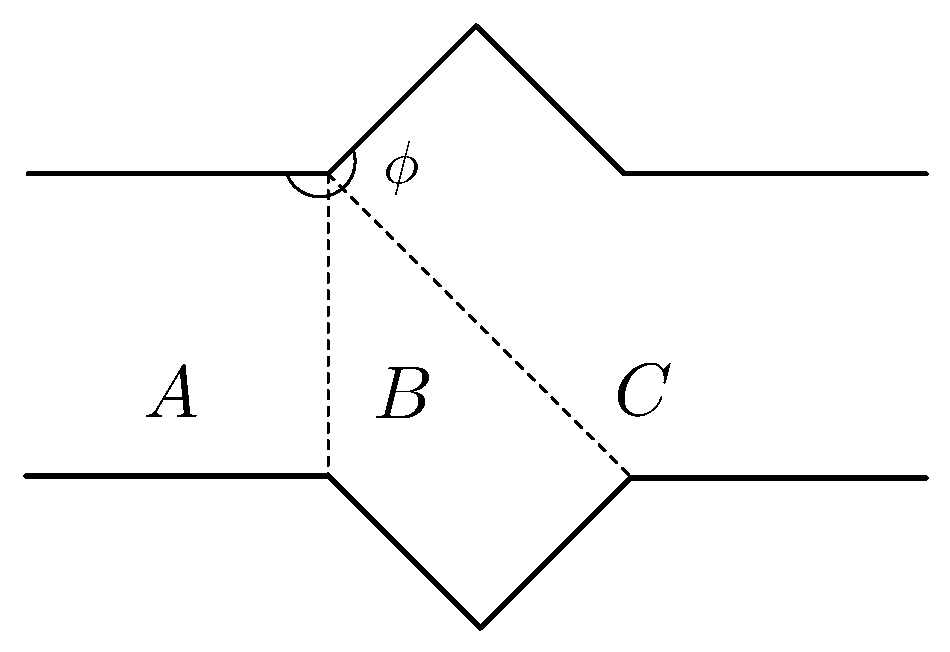
\includegraphics[scale=0.45]{Figures/WallCase.pdf} 
\caption{}\label{fig:wallcase}
\end{figure}

\subsection{The force at doorways}
We encountered a problem when dealing with doors. The problem arises because 
the door is constructed by two free endpoints and pedestrians feel a repulsion 
force from these points according to section \ref{wallEndpoints}. This means 
that a pedestrians trying to exit throw the door will feel a repulsive force 
from the walls which prevent him from walking throw the door. The second he 
passes throw the door he will be pushed forward and accelerate which is unwanted 
behaviour. This we resolved by removing the force from free endpoint when:

\begin{equation}
\| y cos(\alpha) - w \| > R
\end{equation}

This creates what we could call a "non repulsion zone" see figure(Mikkel Lav Tegning!).
In rare cases it could happen that a pedestrian is trying to exit the room and he feels 
no repulsion because he is in the "non repulsive zone", he is then pushed sideways out 
of the "non repulsion zone" and suddenly he will feel a great repulsive force because 
he first "discovers" it when he is very close to the wall see figure(Mikkel Lav Tegning!).

\subsection{The tangential force}
When observing a crowed it could seem as if friction between pedestrians should play 
an important role in the croweds dynamics. This is further confirmed in (ARTICLE) (ARTICLE). 
Here a force vector standing tangent to the circumference of pedestrians. This force 
represents the friction arising when pedestrians touch each other. This fenomena has 
proven to make more accurate predictions.


\subsection{The repulsive force between agents in $ \Re ^{3}$}
From the given formula for calculating the repulsive force between agents in the 
description of the model, the part calculating the force to keep the personal space 
can be omitted when the agents are rather close to each other, then the calculation 
can be reduced as Equation (\ref{eq:re}).

\begin{equation}\label{eq:re}
\overrightarrow{f_{\alpha\beta}}(t) = A_{\alpha}^{2} exp\left[ \frac{r_{\alpha\beta} - d_{\alpha}\beta}{B_{\alpha}^{2}}\right]  \overrightarrow{n_{\alpha\beta}}
\end{equation}

Taking the norms of both sides of Equation (\ref{eq:re}), we can draw the relation 
between the value of $\overrightarrow{f_{\alpha\beta}}(t)$ and $d_{\alpha \beta}$, 
as in Figure (\ref{fig:physicalinteraction})
\\
\begin{figure}
\centering
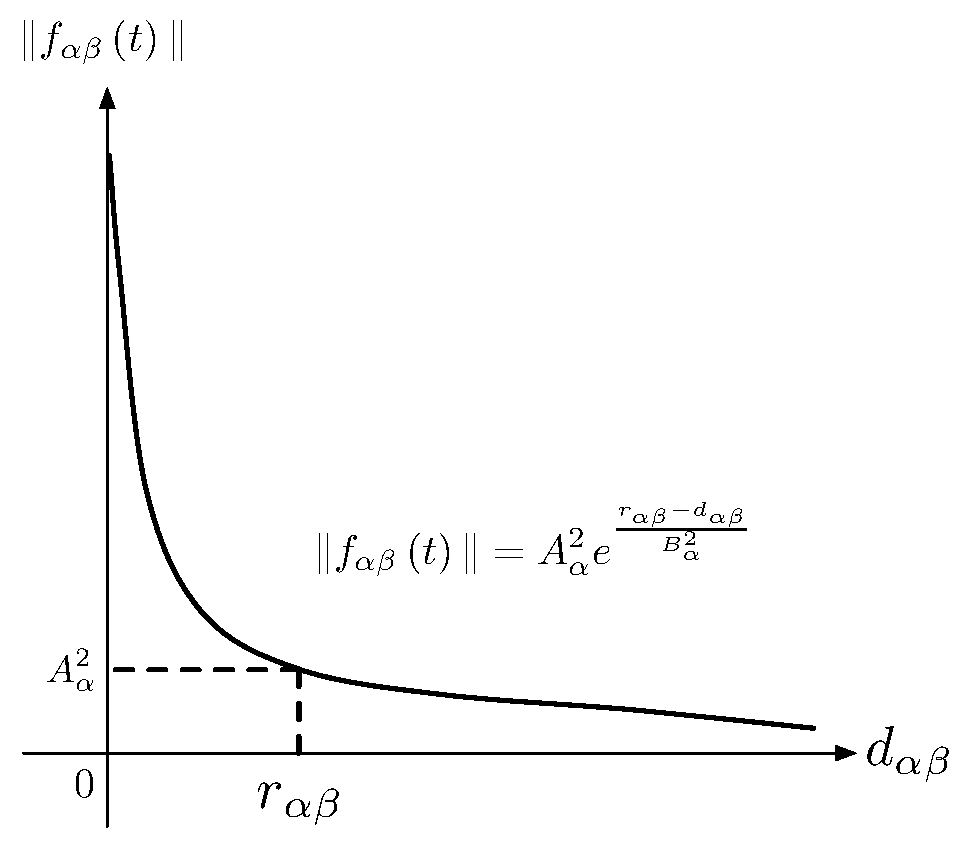
\includegraphics[scale=0.45]{Figures/physicalinteraction.pdf} 
\caption{The function about the interaction force $\vec{f_{\alpha\beta}}(t)$ and the distance between two agents
$d_{\alpha\beta}$ }\label{fig:physicalinteraction}
\end{figure}

There is one intersection of the graph and the axis $ \left( 0, A_{\alpha}^{2} exp\left( \frac{r_{\alpha\beta} }{B_{\alpha}^{2}}\right)  \right) $. 
If put into the constants, we will be able to get a maximum value of $ f_{\alpha\beta}(t) $, 
since the distance between agents cannot be negative. Here we set $ A_{\alpha}^{2} = 3 m/s^{2} $, 
$ r_{\alpha\beta} = 0.6 m $, and $ B_{\alpha}^{2} = 0.2 m $, so $ f_{\alpha\beta}(t)^{max} \doteq 60 m/s^{2} $, 
which is about six times the gravitational acceleration and represents a rather 
large force between agents (as large as six person's weight).

However, we notice that the effective part of the force calculated above is only the horizontal 
component that enables the agent to move horizontally in the plane where we do the simulation, 
but the reality is that the agents sometimes are also able to move vertically, for example, 
by stepping upon other people when they cannot take the pushing force from the surrounding agents. 
When that happens, the horizontal component of the repulsive force becomes smaller even if 
$d_{\alpha\beta}$ is kept the same.	
Therefore, a qualitative modification of dependence between $ f_{\alpha\beta}(t) $ 
and $ d_{\alpha\beta} $ could be:

\begin{figure}[hb]   
\centering
    {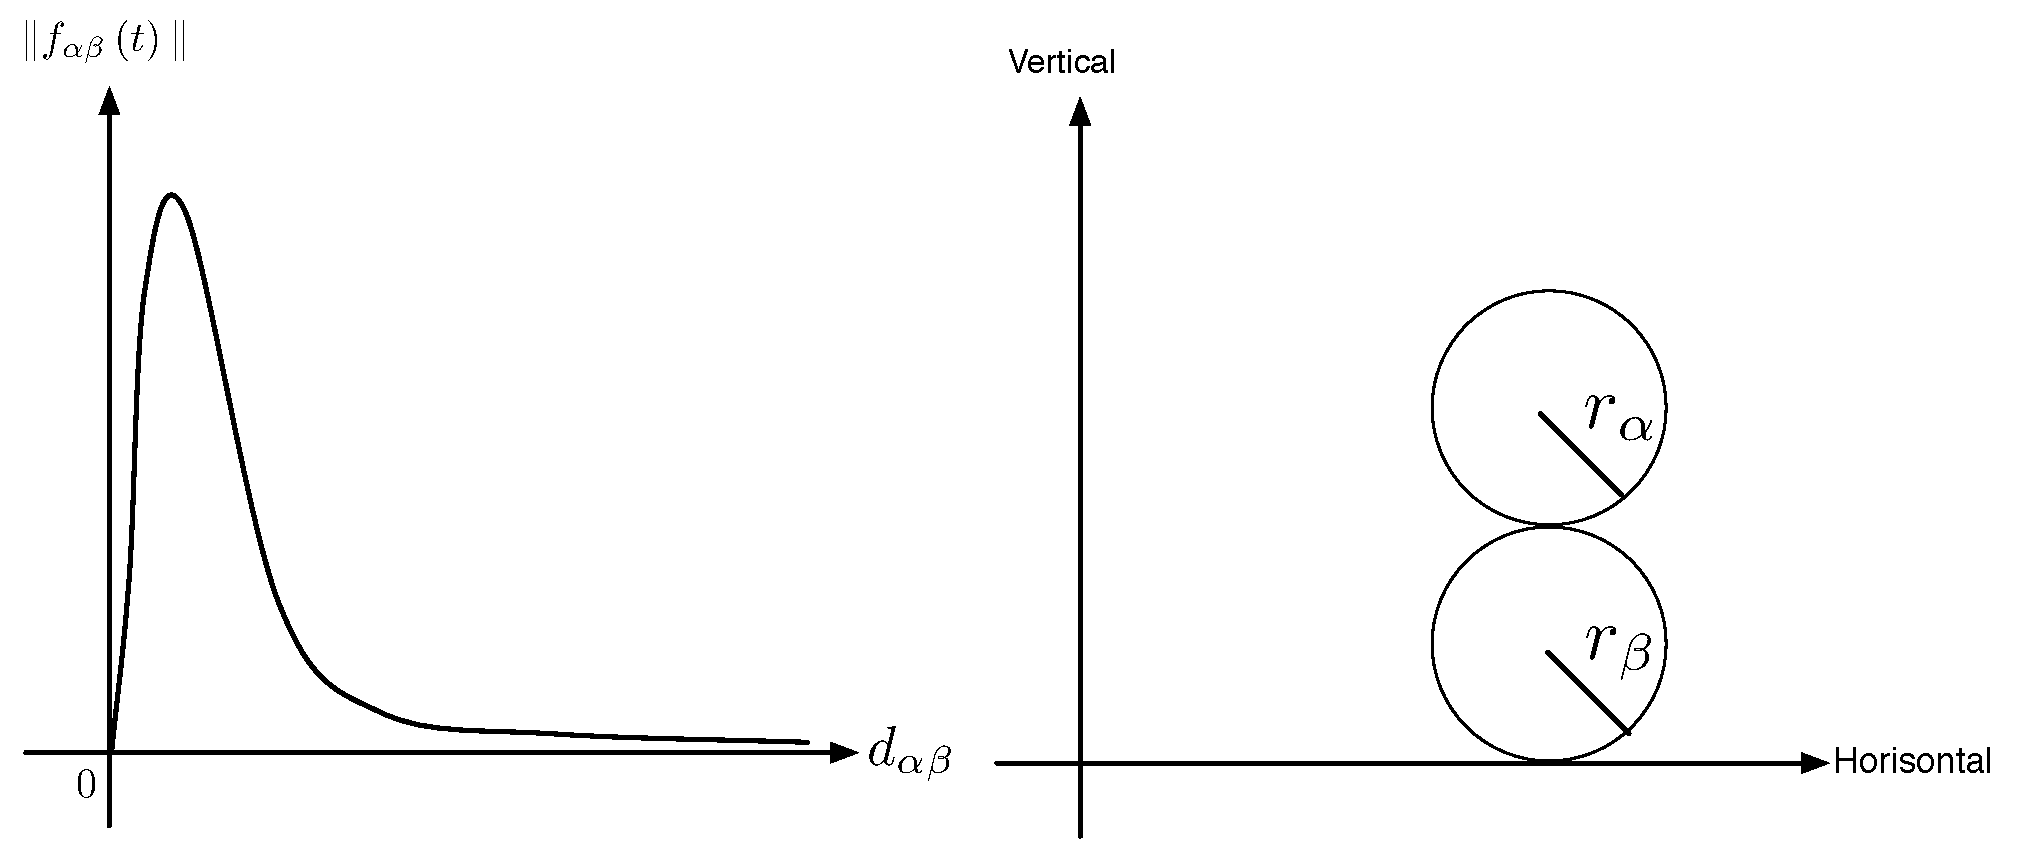
\includegraphics[scale=0.35]{Figures/ForceOverlapping.pdf}} 
    \caption{}
    \label{forceoverlapping}
\end{figure}

\subsection{Use social force in further calculation}
use the value of forces to predict, as they are partly not real forces, the measurement 
does not reflect the reality in some range.
